\section{Date: 2026-08-13}
\noindent \textbf{Series ID: IV1312} 

\noindent This series is titled Import Price Index (Balance of Payments): Air Freight for Asia and has a frequency of Monthly. The units are Index 2000=100 and the seasonal adjustment is Not Seasonally Adjusted.The observation start date is 1990-09-01 and the observation end date is 2026-06-01.The popularity of this series is 3. \\ 

\noindent \textbf{Series ID: IHLIDXUSTPFOPRSE} 

\noindent This series is titled Food Preparation and Service Job Postings on Indeed in the United States and has a frequency of Daily, 7-Day. The units are Index Feb, 1 2020=100 and the seasonal adjustment is Seasonally Adjusted.The observation start date is 2020-02-01 and the observation end date is 2026-08-07.The popularity of this series is 6. \\ 

\subsection{Raw Regression}
\noindent Regresses the two series against each other directly. A significant result here can come just as easily from both series sharing a long-run trend as from any real relationship.

\begin{center}
\begin{tabular}{lclc}
\toprule
\textbf{Dep. Variable:}      & value\_fred\_IHLIDXUSTPFOPRSE & \textbf{  R-squared:         } &     0.023   \\
\textbf{Model:}              &              OLS              & \textbf{  Adj. R-squared:    } &     0.010   \\
\textbf{Method:}             &         Least Squares         & \textbf{  F-statistic:       } &     1.750   \\
\textbf{Date:}               &        Thu, 13 Aug 2026       & \textbf{  Prob (F-statistic):} &    0.190    \\
\textbf{Time:}               &            12:40:03           & \textbf{  Log-Likelihood:    } &   -335.82   \\
\textbf{No. Observations:}   &                 76            & \textbf{  AIC:               } &     675.6   \\
\textbf{Df Residuals:}       &                 74            & \textbf{  BIC:               } &     680.3   \\
\textbf{Df Model:}           &                  1            & \textbf{                     } &             \\
\textbf{Covariance Type:}    &           nonrobust           & \textbf{                     } &             \\
\bottomrule
\end{tabular}
\begin{tabular}{lcccccc}
                             & \textbf{coef} & \textbf{std err} & \textbf{t} & \textbf{P$> |$t$|$} & \textbf{[0.025} & \textbf{0.975]}  \\
\midrule
\textbf{const}               &      95.2838  &       12.490     &     7.629  &         0.000        &       70.398    &      120.170     \\
\textbf{value\_fred\_IV1312} &       0.0574  &        0.043     &     1.323  &         0.190        &       -0.029    &        0.144     \\
\bottomrule
\end{tabular}
\begin{tabular}{lclc}
\textbf{Omnibus:}       &  8.845 & \textbf{  Durbin-Watson:     } &    0.102  \\
\textbf{Prob(Omnibus):} &  0.012 & \textbf{  Jarque-Bera (JB):  } &    8.702  \\
\textbf{Skew:}          & -0.813 & \textbf{  Prob(JB):          } &   0.0129  \\
\textbf{Kurtosis:}      &  3.319 & \textbf{  Cond. No.          } & 1.54e+03  \\
\bottomrule
\end{tabular}
%\caption{OLS Regression Results}
\end{center}

Notes: \newline
 [1] Standard Errors assume that the covariance matrix of the errors is correctly specified. \newline
 [2] The condition number is large, 1.54e+03. This might indicate that there are \newline
 strong multicollinearity or other numerical problems.

\begin{figure}
\centering
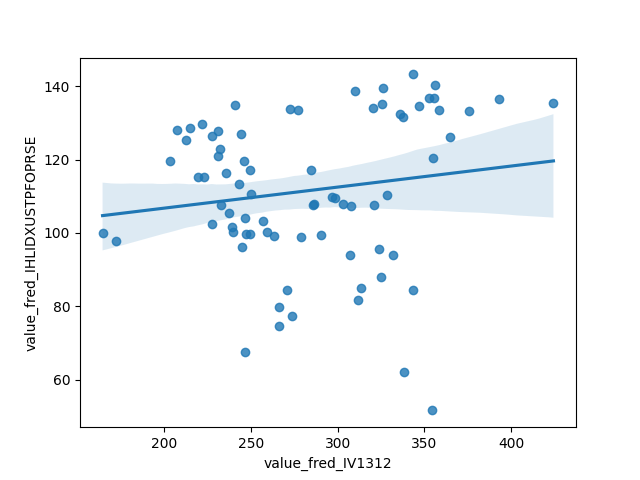
\includegraphics[scale = 0.9]{plots/plot_2026-08-13.png}
\caption{Raw Regression Plot for 2026-08-13}
\end{figure}
\newpage
\subsection{Detrended Regression}
\noindent Regresses the residuals of each series after removing its own linear time trend, so a shared trend can no longer drive the result on its own. A relationship that stays significant here is better evidence of a genuine link between the two series.

\begin{center}
\begin{tabular}{lclc}
\toprule
\textbf{Dep. Variable:}                 & value\_fred\_IHLIDXUSTPFOPRSE\_detrended & \textbf{  R-squared:         } &     0.034   \\
\textbf{Model:}                         &                   OLS                    & \textbf{  Adj. R-squared:    } &     0.021   \\
\textbf{Method:}                        &              Least Squares               & \textbf{  F-statistic:       } &     2.578   \\
\textbf{Date:}                          &             Thu, 13 Aug 2026             & \textbf{  Prob (F-statistic):} &    0.113    \\
\textbf{Time:}                          &                 12:40:03                 & \textbf{  Log-Likelihood:    } &   -335.22   \\
\textbf{No. Observations:}              &                      76                  & \textbf{  AIC:               } &     674.4   \\
\textbf{Df Residuals:}                  &                      74                  & \textbf{  BIC:               } &     679.1   \\
\textbf{Df Model:}                      &                       1                  & \textbf{                     } &             \\
\textbf{Covariance Type:}               &                nonrobust                 & \textbf{                     } &             \\
\bottomrule
\end{tabular}
\begin{tabular}{lcccccc}
                                        & \textbf{coef} & \textbf{std err} & \textbf{t} & \textbf{P$> |$t$|$} & \textbf{[0.025} & \textbf{0.975]}  \\
\midrule
\textbf{const}                          &   -1.576e-11  &        2.316     & -6.81e-12  &         1.000        &       -4.614    &        4.614     \\
\textbf{value\_fred\_IV1312\_detrended} &       0.0727  &        0.045     &     1.605  &         0.113        &       -0.018    &        0.163     \\
\bottomrule
\end{tabular}
\begin{tabular}{lclc}
\textbf{Omnibus:}       &  4.621 & \textbf{  Durbin-Watson:     } &    0.113  \\
\textbf{Prob(Omnibus):} &  0.099 & \textbf{  Jarque-Bera (JB):  } &    4.541  \\
\textbf{Skew:}          & -0.592 & \textbf{  Prob(JB):          } &    0.103  \\
\textbf{Kurtosis:}      &  2.825 & \textbf{  Cond. No.          } &     51.1  \\
\bottomrule
\end{tabular}
%\caption{OLS Regression Results}
\end{center}

Notes: \newline
 [1] Standard Errors assume that the covariance matrix of the errors is correctly specified.

\begin{figure}
\centering
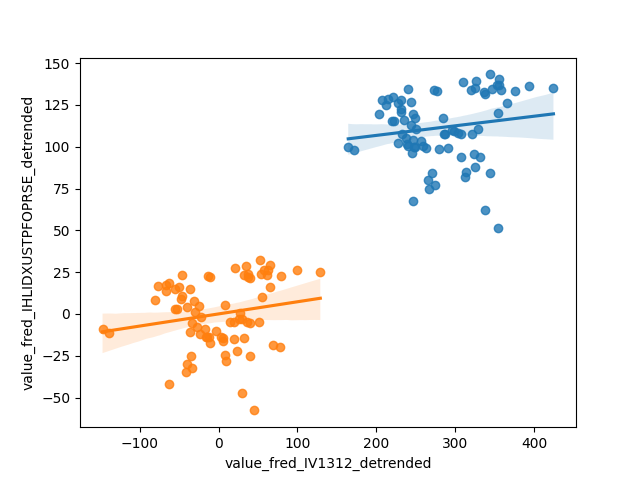
\includegraphics[scale = 0.9]{plots/plot_2026-08-13_detrended.png}
\caption{Detrended Regression Plot for 2026-08-13}
\end{figure}
\newpage
